\documentclass[10pt]{article}
\usepackage{amsmath}
\usepackage{graphicx}
\usepackage{hyperref}
\usepackage[utf8]{inputenc}
\usepackage[spanish]{babel}
\usepackage[margin=2.5cm]{geometry}
\usepackage{amsfonts}
\usepackage{listings}
\usepackage{textcomp}
\usepackage{float}

\title{Pig.}
\author{Néstor Rodríguez Vico - \href{mailto:nrv23@correo.ugr.es}{nrv23@correo.ugr.es}}
\date{\today}

\begin{document}
\maketitle

\setlength{\belowdisplayskip}{5pt} 
\setlength{\belowdisplayshortskip}{5pt}
\setlength{\abovedisplayskip}{5pt} 
\setlength{\abovedisplayshortskip}{5pt}

\section{Origen de los datos.}

El dataset empleado es un dataset sinteético montado con \textit{Python} de forma aleatoria para representar la solución a un problema que cualquier empresa de desarrollo software puede tener. El dataset usado es sintético ya que no puedo usar datos reales de la empresa en la que trabajo por temas de confidencialidad, pero la esencia y la idea representada es la misma. \\

Cualquier producto software tiene un ciclo de desarrollo en el cual podemos, para este caso en particular, destacar dos etapas: el desarrollo del producto y el testeo del mismo. Cuando se trabaja en un software de gran tamaño y bastante complejo, la segunda etapa comentada es primordial. \\

A pesar de que el proceso de testeo de un producto es priomordial, es una tarea compleja, ya que hay que testear todas las partes de un software, las interconexiones de dichas partes y todas las casuísticas posibles, lo cúal hace dicha tarea bastante tediosa y compleja para ser realizada por un humano. Para ello, surgen los tests automátizados. Esto es, una técnica que permite, mediante código, crear tests para probar el producto software en cuestión. \\

Una vez conocemos esta posibilidad, surge la cuestión de como usarlos. La metodología a seguir cuando hay que modificar una pieza software es añadir una nueva funcionalidad o corregir una existente y programar los tests asociados a los cambios producidos. A continuación, se deben ejecutar todos los tests disponibles para asegurarnos que, los cambios introducidos, no han roto ninguna otra parte de nuestro código. Es decir, los tests existen para asegurarnos que, en un futuro, cuando hagamos cambios sobre nuestro software, el funcionamiento del mismo no ha cambiado. \\

Para automatizar aún más el proceso de testeo de un producto, surgen herramientas de Integración Continua (\textit{Continuous Integration}) como pueden ser \href{https://travis-ci.org/}{Travis CI} o \href{https://jenkins.io/}{Jenkins}. La idea de esta herramientas es, conectarlas a un repositorio de código y que cuando haya un \textit{push} a ese repositorio, se ejecutan todos los tests disonibles generando una salida que indica como ha ido la ejecucion de los mismos. De esta manera, cuando un desarrollador quiere modificar un software, lo que debe hacer es añadir su código y sus tests, hacer un \textit{push} al repositorio y esperar a que los tests hayan terminado de ejecutar en \href{https://travis-ci.org/}{Travis CI} o \href{https://jenkins.io/}{Jenkins} para ver el resultado de los mismos. \\

Para una empresa u organización en la que se manejan varios productos software, es relevante tener un estudio de como han ido ejecutando tus tests a lo largo del tiempo, los resultados de los mismos. De esta necesidad, surge la base de datos empleada en esta práctica.

\section{Estructura de los datos.}

La base de datos elegida tiene las siguientes columnas: 

\begin{itemize}
	\item \textbf{id}. Tipo: \textit{entero}. Representa un identificador único.
	\item \textbf{product}. Tipo: \textit{texto}. Producto al que pertenece el test.
	\item \textbf{branch}. Tipo: \textit{texto}. Rama del repositorio donde se encuentra el test ejecutado.
	\item \textbf{date}. Tipo: \textit{texto}. Representa la fecha de ejecución de los tests.
	\item \textbf{run\_number}. Tipo: \textit{entero}. Representa el identificador \href{https://travis-ci.org/}{Travis CI} o \href{https://jenkins.io/}{Jenkins} de la ejecución donde se han ejecutado los tests.
	\item \textbf{test\_area}. Tipo: \textit{texto}. Los tests pueden estar asociados a una área del producto que testean.
	\item \textbf{test\_type}. Tipo: \textit{texto}. Los testes pueden ser de interfaz (\textit{UI test}), tests unitarios (\textit{Unit Test}) o tests de sistema (\textit{System Test.}).
	\item \textbf{class\_name}. Tipo: \textit{texto}. Clase a la que pertenece el tests.
	\item \textbf{method\_name}. Tipo: \textit{texto}. Nombre del método que ejecuta el test.
	\item \textbf{elapsed\_time\_sec}. Tipo: \textit{número real}. Tiempo de ejecución del tests.
	\item \textbf{status}. Tipo: \textit{texto}. Representa el resultado del test, puede ser \textit{PASSDED}, \textit{FAILED} o \textit{ABORTED}.
	\item \textbf{error}. Tipo: \textit{texto}. En el caso de que el test sea \textit{FAILED} o \textit{ABORTED}, tenemos almacenada información del porqué ha fallado el test.
\end{itemize}

\section{Preparación del experimento.}

Primero, debemos cargar los en \textit{hdfs}. Para ello, ejecutamos el comando:

\begin{lstlisting}[frame=single, language=bash, xleftmargin=.25in, basicstyle=\small, upquote=true, breaklines = true]
hdfs dfs -put tests.csv /user/impala/
\end{lstlisting}

A continuación, entramos a la shell de pig con:

\begin{lstlisting}[frame=single, language=bash, xleftmargin=.25in, basicstyle=\small, upquote=true, breaklines = true]
pig
\end{lstlisting}

A continuación, cargamos los datos:

\begin{lstlisting}[frame=single, language=bash, xleftmargin=.25in, basicstyle=\small, upquote=true, breaklines = true]
tests = load '/user/impala/tests.csv' using PigStorage(',') AS (
	id: int,
	product: chararray,
	branch: chararray,
	date: chararray,
	run_number: int,
	test_area: chararray,
	test_type: chararray,
	class_name: chararray,
	method_name: chararray,
	elapsed_time_sec: float,
	status: chararray,
	error: chararray
);
\end{lstlisting}

A continuación, para verificar que todo ha funcionado correctamente, vamos a mostrar los datos por pantalla

\begin{lstlisting}[frame=single, language=sql, xleftmargin=.25in, basicstyle=\small, upquote=true, breaklines = true]
dump tests
\end{lstlisting}

\section{Consultas.}

\subsection{Proyección.}

A continuación, vamos a quedarnos la información relevante para nuestro problema:

\begin{lstlisting}[frame=single, xleftmargin=.25in, basicstyle=\small, upquote=true, breaklines = true]
informacion_relevante = FOREACH tests GENERATE product, branch, date, class_name, method_name, status;
\end{lstlisting}

\subsection{Selección.}

A continuación, quitamos las ejecuciones que son antiguas:

\begin{lstlisting}[frame=single, xleftmargin=.25in, basicstyle=\small, upquote=true, breaklines = true]
ultima_informacion_relevante = FILTER informacion_relevante BY date matches '.*2019-01-10 .*';
\end{lstlisting}

\subsection{Agrupamiento y resúmenes de información.}

Finalmente, calculamos el número de tests fallados, el número de tests totales y porcentaje de tests fallados en cada rama de cada producto:

\begin{lstlisting}[frame=single, xleftmargin=.25in, basicstyle=\small, upquote=true, breaklines = true]
data_grouped = GROUP ultima_informacion_relevante BY (product, branch);

solucion = FOREACH data_grouped {
	failed_bag = FILTER ultima_informacion_relevante BY status == 'FAILED';
	GENERATE group, COUNT(failed_bag) as failed_counter, 
	COUNT(ultima_informacion_relevante) as total_counter, 
	(double) COUNT(failed_bag) * 100.0 / (double) COUNT(ultima_informacion_relevante);
};

dump solucion;
\end{lstlisting}

\begin{figure}[H]
	\centering
	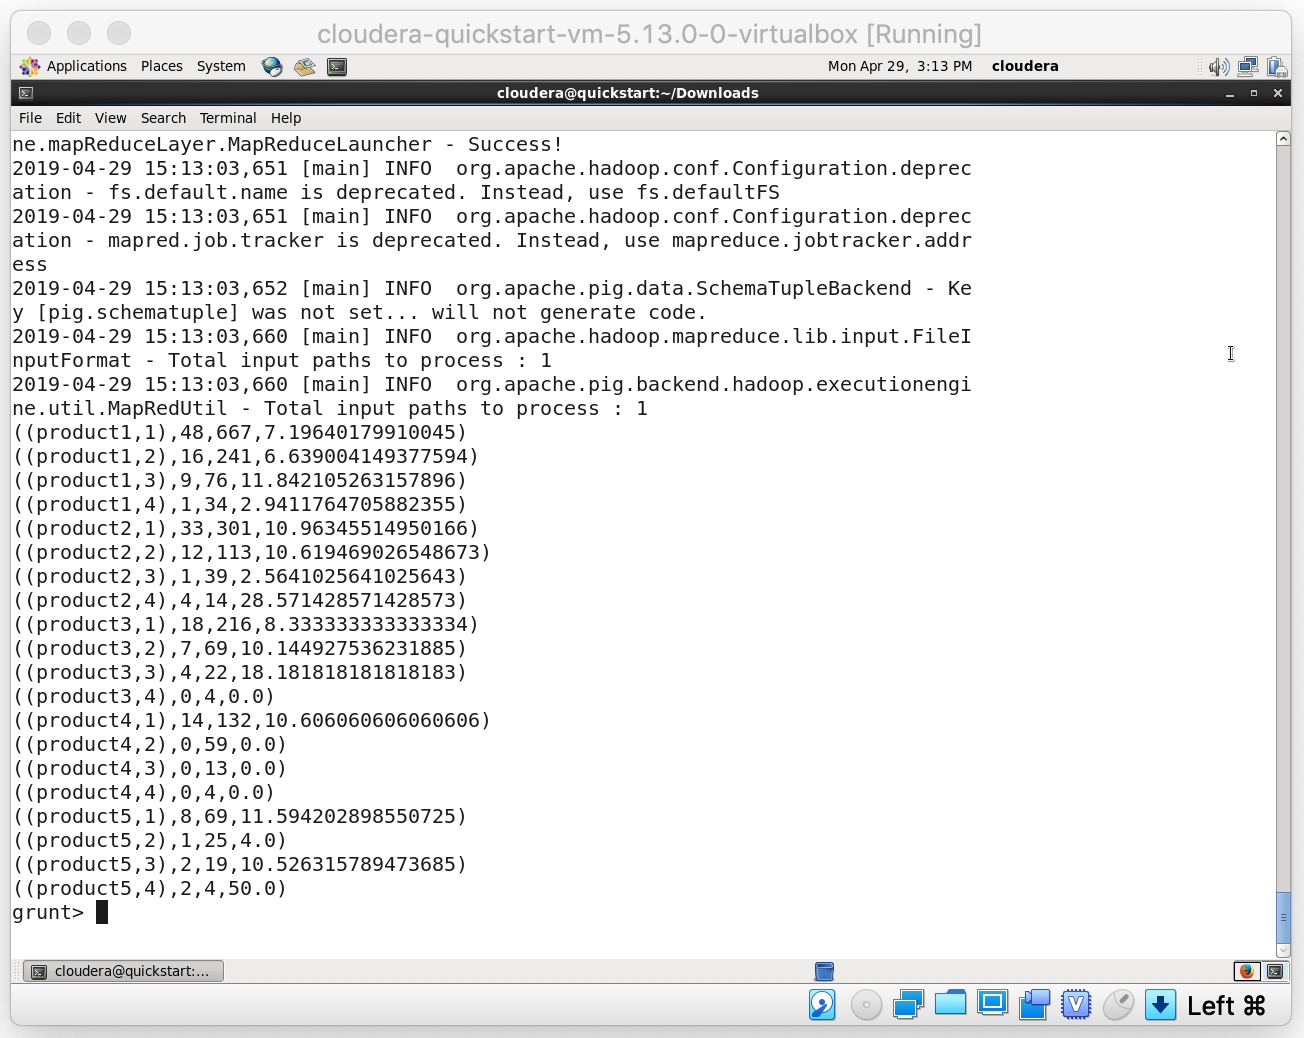
\includegraphics[width=0.7\linewidth]{images/sol.png}
\end{figure}
\end{document}